%%%%%%%%%%%%%%%%%%%%%%%%%%%%%%%%%%%%%%%%%%%%%%%%%%%%%%%%%%%%%%%%%%%%%%%
% BAB 3
%%%%%%%%%%%%%%%%%%%%%%%%%%%%%%%%%%%%%%%%%%%%%%%%%%%%%%%%%%%%%%%%%%%%%%%


% TO DO: Parameter uji

\mychapter{3}{BAB 3 METODOLOGI}

Penelitian ini menggunakan model berbasis LSTM untuk memprediksi kelas pada detak jantung. Model ini kemudian diterapkan pada beberapa perangkat dan diuji dengan menggunakan data detak jantung yang diambil langsung menggunakan sensor ECG. Gambar \ref{fig:diagram-alir} menunjukkan metodologi yang digunakan pada penelitian ini. 
Penelitian dimulai dengan studi literatur untuk mendapatkan informasi yang dibutuhkan. Kemudian dilakukan pengumpulan data detak jantung yang akan digunakan dalam penelitian. Data tersebut kemudian diproses dengan melakukan \textit{preprocessing} untuk menghilangkan \textit{noise} dan normalisasi. Setelah itu, dilakukan ekstraksi fitur dengan menggunakan RR-Interval. Fitur tersebut kemudian digunakan untuk melatih model LSTM. Model tersebut kemudian diimplementasikan pada beberapa perangkat dan diuji dengan menggunakan data detak jantung yang diambil langsung menggunakan sensor ECG. Hasil dari pengujian tersebut kemudian dianalisis dan dibahas.

% TO DO: alur penelitian
% studi literatur, pengumpulan data, preprocessing data, ekstraksi fitur, pembuatan model, implementasi, pengujian, pembahasan

% \begin{figure}[tph]
%   \centering
%   \includegraphics[width=.45\linewidth]{./img/lstm-Page-1.drawio.pdf}
%   \caption{Alur penelitian}
%   \label{fig:diagram-alir}
% \end{figure}

\section{Pengumpulan Data}
\label{subsec: metodologi-pengumpulan-data}


Data yang digunakan untuk melakukan pelatihan pada penelitian ini diperoleh dari dataset publik \textit{MIT‐BIH arrhythmia database} \parencite{moodyImpactMITBIHArrhythmia2001}. Dataset tersebut terdiri dari 48 data yang diambil dari 47 pasien. Pada dataset tersebut, data 102, 104, 107, dan 217 tidak digunakan karena berisi data detak jantung yang dipacu. Setiap rekaman memiliki panjang 30 menit dan terdiri dari dua kanal. Pada penelitian ini, hanya satu kanal yang digunakan, yaitu kanal \textit{Modified Lead II}.
Tiap detak jantung pada dataset tersebut telah diberi label dan anotasi oleh para ahli. Anotasi tersebut dapat dipetakan menjadi kelas sesuai dengan kelas rekomendasi AAMI, yaitu N, SVEB, VEB, F, dan Q \parencite{associationfortheadvancementofmedicalinstrumentationTestingReportingPerformance1998}. Pemetaan tersebut dapat dilihat pada Tabel \ref{tab:aami-label}.

% Ini tidak dibahas detail
% cukup penjelasan narasi singkat
% TO DO: pindah ke bab 2

\begin{table}[h]
	\caption{Kelas Rekomendasi AAMI dan Label pada MIT-BIH}
	\begin{center}
		\begin{tabular}{c @{\hspace{1cm}} c}
			\hline
			AAMI                              & MIT-BIH       \\
			\hline
			Normal (N)                        & N, L, R, e, j \\
			Supraventricular Ectopic Beat (S) & A, a, J, S    \\
			Ventricular Ectopic Beat (V)      & V, E          \\
			Fusion (F)                        & F             \\
			Unknown (Q)                       & /, f, Q       \\
			\hline
		\end{tabular}
	\end{center}
	\label{tab:aami-label}
\end{table}

\section{\emph{Preprocessing} Data}
\label{subsec: metodologi-preprocessing-data}

\textit{Preprocessing} dilakukan untuk memastikan kualitas dan keandalan data yang digunakan dalam proses pelatihan model. \textit{Preprocessing} yang dilakukan yaitu penghapusan \textit{baseline wander} (BW), penghapusan \textit{noise} berfrekuensi tinggi, dan normalisasi. \textit{Baseline wander} atau BW merupakan \textit{noise} berfrekuensi rendah yang terdapat pada ECG. BW dapat disebabkan oleh beberapa faktor, seperti pernapasan, elektroda yang bermuatan listrik, dan gerakan dari pasien \parencite{lenisComparisonBaselineWander2017}. Setelah dilakukan penghapusan BW, tahap selanjutnya adalah menghilangkan \textit{noise} dengan frekuensi tinggi. Setelah \textit{noise} berfrekuensi tinggi dihilangkan, data dinormalisasi untuk menghindari perbedaan skala. Normalisasi yang dilakukan yaitu \textit{Z-score normalization}. Gambar \ref{fig:sebelum-prep} menunjukkan data sebelum dilakukan \textit{preprocessing}, sedangkan Gambar \ref{fig:setelah-prep} menunjukkan data setelah dilakukan \textit{preprocressing}.

\begin{figure}[H]
    \centering
    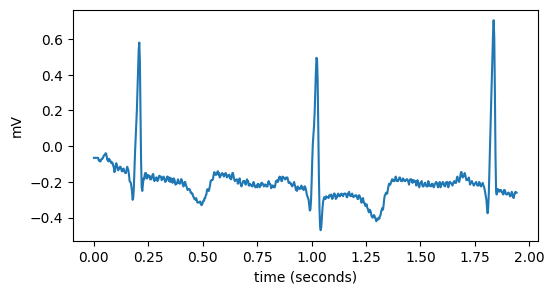
\includegraphics[width=0.6\linewidth]{./img/sebelum_prep.png}
	\caption{Data sebelum \textit{preprocessing}}
	\label{fig:sebelum-prep}
\end{figure}

\begin{figure}[H]
  \centering
  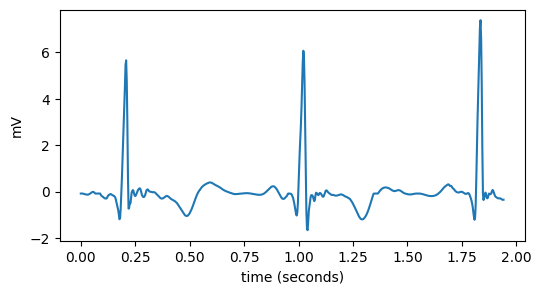
\includegraphics[width=0.6\linewidth]{./img/setelah_prep.png}
  \caption{Data setelah \textit{preprocessing}}
  \label{fig:setelah-prep}
\end{figure}


\section{Ekstraksi Fitur}
\label{subsec: metodologi-ekstraksi-fitur}

Kami menggunakan RR-Interval sebagai fitur dalam penelitian ini. RR-Interval adalah jarak antara dua titik R pada sinyal ECG. Visualisasi dari RR-Interval ditunjukkan oleh Gambar \ref{fig:rri}. Dari interval RR ini, kami mengekstraksi 9 fitur, yaitu RR0, RR-1, RR+1, RR0/avgRR, tRR0, RR-1/avgRR, RR-1/RR0, RR+1/avgRR, dan RR+1/RR0 \parencite{pramukantoroHeartbeatClassifierContinuous2022}. Tabel \ref{tab:rri} menunjukkan deskripsi lengkap dari setiap fitur. Ekstraksi dilakukan dengan jendela sepanjang 42 data. Rata-rata RR-Interval (avgRR) merupakan rata-rata dari 42 data, termasuk RR-0. 

\begin{figure}[H]
  \centering
  \includegraphics[scale=.7]{img/lstm-Page-7.drawio.pdf}
  \caption{RR-Interval}
  \label{fig:rri}
\end{figure}

\begin{table}[H]
  \caption{Deskripsi RR-Interval}
\begin{center}
\footnotesize
\begin{tabular}{c @{\hspace{1cm}} c}
\hline
Fitur & Deskripsi\\
\hline
RR0 & Nilai RRi saat ini\\
RR-1 & Nilai RRi sebelumnya\\
RR+1  & Nilai RRi selanjutnya\\
RR0/avgRR & Nilai RRi saat ini dibagi dengan rata-rata 42 RRi sebelumnya\\
tRR0  & (RRi saat ini - rata-rata RRi) / stddevRRi\\
RR-1/avgRR & Nilai RRi sebelumnya / rata-rata RRi\\
RR-1/RR0 & Nilai RRi sebelumnya / RRi saat ini\\
RR+1/avgRR & Nilai RRi selanjutnya / rata-rata RRi\\
RR+1/RR0 & Nilai RRi selanjutnya / RRi saat ini\\
\hline
\end{tabular}
\end{center}
\center
Sumber: \textcite{pramukantoroHeartbeatClassifierContinuous2022}
\label{tab:rri}
\end{table}

% considering cuma pakai lstm256 tapi dengan fitur lain
\section{Pembuatan Model LSTM}
\label{subsec: metodologi-pembuatan-model-lstm}
Pada tahap ini, penulis membuat model berbasis LSTM yang akan digunakan untuk melakukan klasifikasi detak jantung. 
% Dalam penelitian ini, 
Terdapat tiga jenis model yang akan digunakan pada penelitian, yaitu \textit{Long Short-Term Memory} (LSTM), \textit{Bidirectional} LSTM (Bi-LSTM), serta LSTM \textit{Fully Convolutional Network} (LSTM-FCN). 
Pembuatan model meliputi pembuatan arsitektur model, pelatihan model, dan evaluasi model.
Model dibuat dengan menggunakan \textit{framework} TensorFlow dan dilatih sebanyak 50 \textit{epoch}.


% LSTM merupakan pengembangan dari \textit{Recurrent Neural Network} (RNN) yang dirancang untuk mengatasi masalah yang umum terjadi pada RNN tradisional, yaitu hilangnya informasi masa lalu \parencite{hochreiterLongShorttermMemory1997}.  LSTM memiliki kemampuan untuk mengingat informasi yang disimpan dalam jangka waktu yang lama. 

\section{Implementasi}
\label{subsec: metodologi-implementasi}

Model yang telah dilatih selanjutnya diimplementasikan pada beberapa perangkat antara lain Raspberry Pi 4 dan Intel NUC untuk menjalankan proses inferensi. Model diimplementasikan dalam bentuk aplikasi berbasis web yang dibuat dengan menggunakan \textit{framework} Flask. Sebelum diimplementasikan, model dioptimasi terlebih dahulu agar dapat beroperasi secara efisien terutama pada perangkat dengan daya komputasi rendah seperti Raspberry Pi. Model dioptimasi dengan cara melakukan konversi ke dalam bentuk TensorFlow Lite (tflite). Model TensorFlow Lite memiliki ukuran yang lebih kecil dan membutuhkan lebih sedikit dependensi dibanding dengan model TensorFlow. Pada proses optimasi, juga dilakukan kuantisasi yang dapat mengurangi penggunaan memori dan mempercepat komputasi
.
% sehingga cocok untuk perangkat dengan spesifikasi rendah seperti Raspberry Pi.

% flowchart aplikasi

\section{Pengujian}
\label{subsec: metodologi-pengujian}

% Pengujian dilakukan pada perangkat Raspberry Pi 3B. Perangkat ini memiliki prosesor ARMv8 quad-core 1,2GHz dan RAM 1GB LPDDR2. Konektivitas perangkat ini didukung dengan 2.4Ghz WiFi serta \textit{ethernet} dengan kecepatan maksimum 100Mbps.
% pindah ke landasan teori

Pengujian dilakukan menggunakan data uji berupa data detak jantung yang diperoleh dari sensor ECG Polar H10. 
%tujuan pengujian
Pengujian dilakukan untuk mengukur tingkat akurasi prediksi serta efisiensi komputasi. 
%metode pengujian
Pengujian dilakukan dengan merekam waktu prediksi serta penggunaan memori ketika melakukan inferensi pada data detak jantung.
Pengujian dilakukan dengan menggunakan data detak jantung sepanjang 10 detik, 1 menit, dan 10 menit. Pengujian dilakukan dengan menggunakan 3 model yang telah dilatih sebelumnya, yaitu LSTM, Bi-LSTM, dan LSTM-FCN. Pengujian dilakukan sebanyak 5 kali untuk setiap \textit{classifier} untuk kemudian diambil nilai rata-rata dari hasil tersebut.

\section{Pembahasan}
\label{subsec: metodologi-pembahasan}

Pada tahap ini, hasil pengujian akan dianalisis secara mendalam.
Hasil pengujian model akan dibandingkan untuk mencari model dengan performa terbaik.
Selain itu, hasil pengujian juga akan dibandingkan dengan hasil penelitian-penelitian sebelumnya.
% Hasil dari pengujian ini akan menjadi subjek utama pembahasan.

\section{Jadwal penelitian}
\label{subsec:label}

\begin{figure}[tph]
%   \centering
%   \includegraphics[width=.7\linewidth]{img/jadwal.png}
%   \caption{Jadwal Penelitian}
%   \label{fig:jadwal-penelitian}
\end{figure}
